\section{Domains with Zero-Cost Actions}
\label{sec:zerocost-domains}
%% best to put openstacks here, considering the connection to the
%% previous section
\pddl{Openstacks}  is a cost
minimization domain introduced in IPC-2006, where the objective is to 
minimize the number of stacks used.
One characteristics of Openstacks is the presence of many zero-cost actions which do not increase the number of stacks, the objective function in this domain. These zero-cost actions creates the problem depicted in \refig{fig:plateau-1}.
% Since 0-cost actions corresponds to 0-cost search edges.
% If such actions are present, the neighbors of the goal nodes could be surrounded by the 0-cost edges.
Since zero-cost actions (edges) allows ``free'' transitions between many neighboring nodes,
the number of neighboring nodes sharing the same $h$ also becomes quite large.
This creates huge heuristic plateaus of $h$, which prevent the standard $h$-based tiebreaking from producing informative guidance within plateau $f=f^*$.

\begin{figure}[htbp]
  \centering
  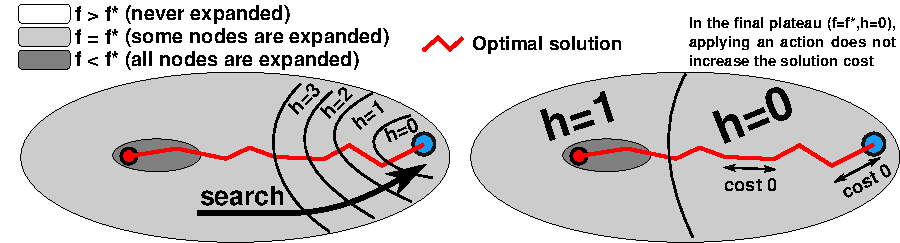
\includegraphics{img/astar/plateau-1.pdf}
 \caption{Search space of \astar and its contour according to $h$. (\textbf{Right}) In positive cost domains, $h$-tiebreaking provides a meaningful guidance. (\textbf{Left}) In domains with 0-cost actions, applying an action may not increase the cost of the path, and thus the region of $h=0$ could be quite large. Thus $h$-tiebreaking fails to provide meaningful guidance.
  }
 \label{fig:plateau-1}
\end{figure}


%% safe to remove these explanation.
% According to \cite{richter2010lama}, \textbf{??????}
% %Richter talks about the failures on openstacks starting around p.167
% \lmcut \cite{Helmert2009} fails to find a good cost
% partitioning with non-zero values, 
% % A detailed discussion of Openstacks domain and poor performance of landmarks is in \cite{richter10lama}, p.167-169.
% and most edges in the abstraction
% space of M\&S \cite{helmert2007flexible} have zero costs.

% XXX I'm commenting out the paragraphs below because:
% (1) A review of heuristic functions for domain-independent learning is not really
% necessary for this AAAI submission. 
% (2) It's better if this paper is not so strongly associated with the ICAPS community only -- this work applies in general to search with A*, and is not strongly tied to almost-perfect heuristics, lmcut, m&s, etc.

Although domains with zero-cost actions are not common in the current set of benchmarks, we argue that such domains are of an important class of models for cost-minimization problems, i.e.,
assigning zero costs make sense from a practical, modeling perspective.
For example, consider the \pddl{driverlog} domain, where the task is to move packages between locations using trucks.
The IPC version of this domain assigns unit costs to all actions. Thus, cost-optimal planning on this domain seeks to minimize the number of steps in the plan.
However, another natural objective function would be the one which minimizes the amount of fuel spent by driving the trucks,
assigning cost 0 to all actions except \pddl{drive-truck}.

% While I agree with the point you're trying to make,
% There is an ugly issue when arguing that current models try to  optimize plan-execution time (i.e., makespan), 
% which is that if we really cared about makespan optimality, we would consider parallel execution of actions whenever possible.
% however, sequential classical planners do not handle parallel actions at all  (recall ACP).
% so arguing this path can only lead to trouble.. Let's try a safer line of argument.
%% For runtime minimization,
%% nonzero positive costs are reasonable because
%% every actions are supposed to consume a fraction of time.
%% However, such formulation is not suitable for general optimization
%% problems.  For example, when you try to minimize the energy consumption
%% by the elevators in \pddl{Elevators} domain, many actions would have zero-cost
%% --- it does not consume electricity for either boarding or leaving the
%% passenger, or moving the elevator down.
%% % 
%% From the practical point of
%% view, cost minimization domains would have wider interest compared to
%% the simple runtime minimization.
%% Also, as shown previously, such domains pose a
%% difficulty to the current heuristic planners due to their large plateaus.

Similarly, for many practical applications, a natural objective is to
optimize the usage of one key consumable resource, e.g., fuel/energy
minimization.  In fact, two of the IPC domains, \pddl{Openstacks} and
\pddl{Cybersec}, which were shown to be difficult for standard tiebreaking
methods in the previous section, both contain many zero-cost actions,
and \textbf{both are based on industrial applications}: \pddl{Openstacks} models
production planning \cite{fink1999applications} and \pddl{Cybersec}
models Behavioral Adversary Modeling System \cite[minimizing decryption,
data transfer, etc.]{boddy2005course}.

Therefore, in this paper, we modified various domains
into cost minimization domains with many zero-cost actions.
Specifically, a domain is modified so that all action schema are assigned
cost 0 except for a few (usually one) action schema which consumes some key resource.
The suffixes in the names of these domains indicate the actions with non-zero costs, e.g., \pddl{elevator-up} is a modified elevator
domain where the \pddl{up} action is assigned non-zero cost (because
elevators are considered to consume energy only when going \pddl{up}), and all other actions have cost 0.
Most of the transportation-type domains are modified to optimize 
energy usage (\pddl{Logistics-fuel}, \pddl{elevator-up} etc.), and  assembly-type domains are modified to minimize resource usage
%% floortile-ink is not shown, so better not to mention it
(\pddl{Woodworking-cut} minimizes wood usage, etc.).

We did not
include domains which have only a single action schema, or which already had many zero-cost actions.
We refer to these 28 new domains as \emph{zerocost domains}.
In detail, they are:
airport-fuel (20), blocks-stack (20), depot-fuel (22), driverlog-fuel (20),
elevators-up (20), floortile-ink (20), freecell-move (20), grid-fuel (5),
gripper-move (20), hiking-fuel (20), logistics00-fuel (28), miconic-up (30),
mprime-succumb (35), mystery-feast (20), nomystery-fuel (20),
parking-movecc (20), pathways-fuel (30), pipesnt-pushstart (20),
pipesworld-pushend (20), psr-small-open (20), rovers-fuel (40),
scanalyzer-analyze (20), sokoban-pushgoal (20), storage-lift (20),
tidybot-motion (20), tpp-fuel (30), woodworking-cut (20),
zenotravel-fuel (20).

The number of instances may be different between the original domain and
the zerocost domain. One such example is \pddl{miconic}, which
originally have 150 instances while our zerocost version have
30 instances.
This is in order to reduce the effect of the difference in the
number of instances in each domain to the overall coverage sum.
In those cases, we sampled the instances evenly from the original set
of instances. For example, we picked p05, p10, ... p150 to select 30
instances.

\subsection{Difference in Problem Characteristics between IPC and Zerocost Domains}

We first tested if these new domains actually poses a new type of challenge to the
standard tiebreaking strategies. Results using \lmcut and \mands
heuristics are shown in \reftbl{tbl:lmcut-zerocost-std} and
\reftbl{tbl:mands-zerocost-std}, respectively. In each table, the left
hand side shows the results in the original domains, and the right hand side
shows the zerocost versions of the domains modified from the same
instances in the left hand side. We did not include the domains whose
number of instances differ from each other.

In both \lmcut and \mands heuristics, we observed a significant
performance difference between the original IPC domains and the zerocost
domains. With \lmcut, the coverage in zerocost domains
was lower in 11 domains, while more instances were solved
in 5 domains. With \mands, the coverage in zerocost domains was lower in 10 domains, while
more instances were solved in 3 domains.

Also, \refig{fig:plateau-zerocost} plots the size of the final plateau of the
zerocost domain instances, with \lmcut heuristics and $h$-tiebreaking. In this plot,
each point shows the total number of nodes in $\plateau{f^*,0}$ vs the
total number of nodes with $f\leq f^*$. Compared to \refig{fig:plateau},
most zerocost domains have larger plateaus even with the help of
$h$-tiebreaking.  Thus, in these cost-minimization problems, the search
strategy within plateaus, i.e., tiebreaking, becomes a yet more critical
factor which determines the search performance.

\begin{table}[htbp]
 \centering
 \setlength{\tabcolsep}{0.2em}
\begin{center}
\begin{tabular}{|lc|ccr|}
 & solved & solved & (difference) & \\
depot(22) & 6 & 6 &  & depot-fuel(22)\\
driverlog(20) & 13 & 8 & (-5) & driverlog-fuel(20)\\
elevators-opt11(20) & 15 & 7 & (-8) & elevators-up(20)\\
floortile-opt11(20) & 6 & 8 & (+2) & floortile-ink(20)\\
grid(5) & 1 & 1 &  & grid-fuel(5)\\
gripper(20) & 6 & 7 & (+1) & gripper-move(20)\\
logistics00(28) & 20 & 16 & (-4) & logistics00-fuel(28)\\
mprime(35) & 21 & 15 & (-6) & mprime-succumb(35)\\
nomystery-opt11(20) & 14 & 10 & (-4) & nomystery-fuel(20)\\
parking-opt11(20) & 1 & 0 & (-1) & parking-movecc(20)\\
pathways(30) & 5 & 5 &  & pathways-fuel(30)\\
rovers(40) & 7 & 8 & (+1) & rovers-fuel(40)\\
scanalyzer-opt11(20) & 10 & 9 & (-1) & scanalyzer-analyze(20)\\
sokoban-opt11(20) & 19 & 18 & (-1) & sokoban-pushgoal(20)\\
storage(30) & 14 & 4 & (-10) & storage-lift(20)\\
tidybot-opt11(20) & 12 & 16 & (+4) & tidybot-motion(20)\\
tpp(30) & 6 & 8 & (+2) & tpp-fuel(30)\\
woodworking-opt11(20) & 10 & 5 & (-5) & woodworking-cut(20)\\
zenotravel(20) & 11 & 7 & (-4) & zenotravel-fuel(20)\\
\end{tabular}
\end{center}

 \caption{
 Coverage comparison (the number of instances solved) 
 between the original instances and the modified zerocost instances,
 using the same configuration and experimental setting (5min, 4GB, \lmcut heuristics).
 This table does not include domains where the total number of instances
 differ in the zerocost domain and the original domain. The results in
 those domains are available in the later sections.
 }
 \label{tbl:lmcut-zerocost-std}
\end{table}

\begin{table}[htbp]
 \centering
 \begin{center}
\begin{tabular}{|lc|cr|}
 & \([f,h,\fifo]\) & \([f,h,\fifo]\) & \\
depot(22) & 6 & 5 & depot-fuel(22)\\
driverlog(20) & 12 & 9 & driverlog-fuel(20)\\
elevators-opt11(20) & 13 & 8 & elevators-up(20)\\
floortile-opt11(20) & 6 & 8 & floortile-ink(20)\\
grid(5) & 2 & 2 & grid-fuel(5)\\
gripper(20) & 20 & 20 & gripper-move(20)\\
logistics00(28) & 20 & 16 & logistics00-fuel(28)\\
mprime(35) & 23 & 21 & mprime-succumb(35)\\
nomystery-opt11(20) & 18 & 16 & nomystery-fuel(20)\\
parking-opt11(20) & 1 & 0 & parking-movecc(20)\\
pathways(30) & 4 & 4 & pathways-fuel(30)\\
rovers(40) & 8 & 8 & rovers-fuel(40)\\
scanalyzer-opt11(20) & 10 & 11 & scanalyzer-analyze(20)\\
sokoban-opt11(20) & 20 & 19 & sokoban-pushgoal(20)\\
storage(30) & 15 & 4 & storage-lift(20)\\
tidybot-opt11(20) & 0 & 0 & tidybot-motion(20)\\
tpp(30) & 7 & 9 & tpp-fuel(30)\\
woodworking-opt11(20) & 7 & 7 & woodworking-cut(20)\\
zenotravel(20) & 12 & 10 & zenotravel-fuel(20)\\
\end{tabular}
\end{center}

 \caption{
 Coverage comparison (the number of instances solved) 
 between the original instances and the modified zerocost instances,
 using the same configuration and experimental setting (5min, 4GB, \mands heuristics).
 This table does not include domains where the total number of instances
 differ in the zerocost domain and the original domain. The results in
 those domains are available in the later sections.
 }
 \label{tbl:mands-zerocost-std}
\end{table}

\begin{figure}[htbp]
  \centering
  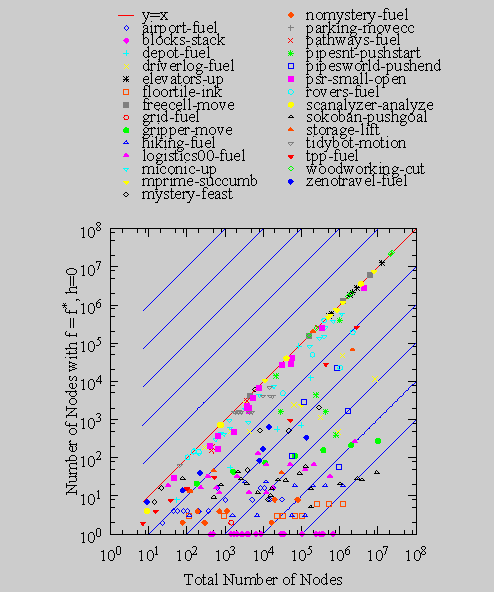
\includegraphics{tables/aaai16-frontier/zerocost/lmcut_frontier-front.pdf}
  \caption{
 The number of nodes with $f=f^*, h=0$ (y-axis), which form
  the final plateau when $h$-based tiebreaking is enabled, compared to
 the total number of nodes in the search space (x-axis) with
 $f\leq f^*$ on 620 instances in our \emph{zerocost domains}.
 The size of final plateaus tends to account for larger portion of the
 entire search space compared to \refig{fig:plateau}.
 This statistics is obtained by running a modified Fast Downward with
 \lmcut which continues searching after the solution is found
 until expanding all nodes with cost $f=f^*$.
 }
 \label{fig:plateau-zerocost}
\end{figure}

\subsection{Discussion on Zerocost Domains}

Note that the difficulty posed by these domains sometimes \emph{cannot}
be tackled by improving the heuristic estimates, or reducing the
underestimation of an admissible heuristic function.  Due to the
existence of 0-cost edges, some non-goal neighbors of a goal node can
legitimately have $h^*=0$. For those nodes,
there are no room for improving the heuristic estimate; Any positive
value causes the heuristics to be inadmissible.

There are two options to improve the search performance in such plateaus
produced by zerocost problems. The first option is to enhance the search
by combining multiple heuristics; It allows the heuristics to be
inadmissible when it is only used for tiebreaking strategy. The obvious
drawback of this strategy is the cost of additional heuristic
computation.

Another option is to perform an efficient
\emph{knowledge-free} search within plateau; It may reuse the effort
that are already spent to guide the search, but does not require
additional effort to compute multiple heuristics.
% Thus, in order to solve zerocost problems more efficiently, the planner
% needs to perform an efficient \emph{knowledge-free} search within a
% large, final plateau. 

In the next section, we first propose and evaluate an implementation of
the second option.  It turns out that a notion of \emph{depth} can have
a significant impact on the performance of knowledge-free search, as
well as a good understanding of the existing tiebreaking strategies.

